%----------------------------------------------------------------------------------------
%	PACKAGES AND THEMES
%----------------------------------------------------------------------------------------
\documentclass[aspectratio=169,xcolor=dvipsnames]{beamer}
\usetheme{SimplePlus}

\usepackage{hyperref}
\usepackage{graphicx} % Allows including images
\usepackage{booktabs} % Allows the use of \toprule, \midrule and \bottomrule in tables
\usepackage{media9}
\usepackage[dvipsnames]{xcolor}

\graphicspath{{./images/}}

%----------------------------------------------------------------------------------------
%	TITLE PAGE
%----------------------------------------------------------------------------------------

\title[short title]{Fair Division} % The short title appears at the bottom of every slide, the full title is only on the title page
\subtitle{Cake Cutting Algorithms: Be Fair if You Can}

\author[Iniyan Joseph] {Iniyan Joseph}

\institute[UTD] % Your institution as it will appear on the bottom of every slide, may be shorthand to save space
{
    University of Texas at Dallas % Your institution for the title page
}
\date{} % Date, can be changed to a custom date


%----------------------------------------------------------------------------------------
%	PRESENTATION SLIDES
%----------------------------------------------------------------------------------------

\begin{document}
% \beamerdefaultoverlayspecification{<+->}

\begin{frame}
    % Print the title page as the first slide
    \titlepage
\end{frame}

\begin{frame}{Overview}
    % Throughout your presentation, if you choose to use \section{} and \subsection{} commands, these will automatically be printed on this slide as an overview of your presentation
    \tableofcontents
\end{frame}

%------------------------------------------------
\section{Introduction to Fair Division}
%------------------------------------------------
\begin{frame}{Meeting 1}
	\begin{block}{Agenda}
		\begin{itemize}
			\item Introduction
			\item Fair Division for n Players
			\begin{itemize}
				\item Banach Knaster
				\item Dubins Spanier
				\item Even Paz
			\end{itemize}
		\end{itemize}
	\end{block}
\end{frame}
%------------------------------------------------
\begin{frame}{Introduction}
	Imagine two people want to share this cake.
	\begin{figure}
		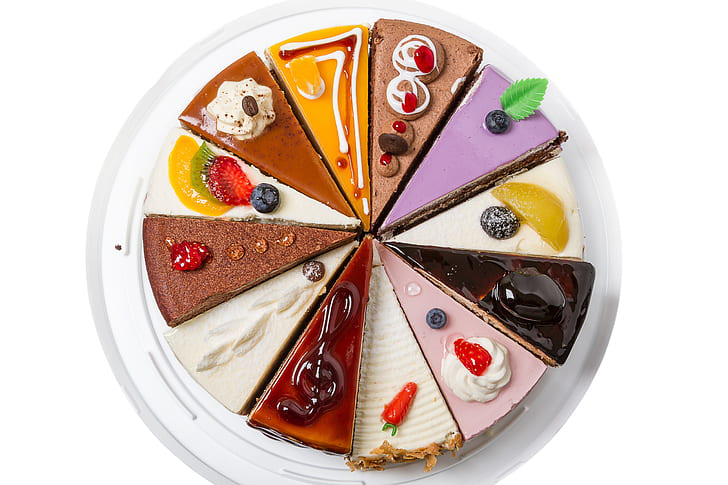
\includegraphics[width=0.75\linewidth]{cakeImage}
	\end{figure}
\end{frame}

%------------------------------------------------
\begin{frame}{Introduction}
    \begin{itemize}
        \item The cake is complicated
        \item The two people may value different parts of the cake differently\pause
        \item Can we come up with an algorithm where both people are happy?
    \end{itemize}
\end{frame}
%------------------------------------------------
\section{Cut and Choose}
%------------------------------------------------
\begin{frame}
	\Huge{\centerline{\textbf{Cut and Choose}}}
\end{frame}
%------------------------------------------------
\begin{frame}{Procedure}
	\begin{enumerate}
		\item Player 1 cuts the cake into what they believe is half
		\item Player 2 chooses the piece which they think is better
	\end{enumerate}
\end{frame}
%------------------------------------------------
\begin{frame}{Proof of Correctness}
	\begin{itemize}
		\item Player 1 recieves $\frac{1}{2}$ of the cake
		\item Player 1 values Player 2's allocation to also be worth $\frac{1}{2}$\pause
		\item Player 2 recieved the piece which they thought was better
		\item Player 2 must value their piece to be at least $\frac{1}{2}$ of the cake
	\end{itemize}
\end{frame}
%------------------------------------------------
\section{Fair Division for $n$}
%------------------------------------------------
\subsection{Banach-Knaster Last Diminisher}
%------------------------------------------------
\begin{frame}
	\Huge{\centerline{\textbf{Banach-Knaster Last Diminisher}}}
\end{frame}
%------------------------------------------------
\begin{frame}{Procedure}
	\begin{enumerate}
		\item Player 1 cuts $\frac{1}{n}$ of the cake
		\item Player 2 through n
		\begin{itemize}
			\item If they believe the piece is worth $> \frac{1}{n}$ of the cake, they may trim it
			\item If they believe the piece is worth $\leq \frac{1}{n}$ of the cake, they may pass it to the next person
		\end{itemize} \pause
		\item The last person to trim the piece recieves it and drops out\pause
		\item Repeat until no players remain
	\end{enumerate}
\end{frame}
%------------------------------------------------
\begin{frame}{Proof of Correctness}
	\begin{itemize}
		\item Cutting a piece to be $> \frac{1}{n}$ can cause further division to be limited to $< \frac{1}{n}$ of the cake
		\item This is most easily seen with an extreme example \pause
		\begin{enumerate}
			\item Person 1 cuts 98\% of the cake, with the goal of taking it for themselves.
			\item After passing the cake around, the last diminisher has only cut the piece down to 97\% of the value of the cake
			\item Person 1 now cannot receive more than 3\% of the cake.
		\end{enumerate}
	\end{itemize}
\end{frame}
%------------------------------------------------
\subsection{Dubins-Spanier Moving Knife}
%------------------------------------------------
\begin{frame}
	\Huge{\centerline{\textbf{Dubins-Spanier Moving Knife}}}
\end{frame}
%------------------------------------------------
\begin{frame}{Procedure}
	\begin{itemize}
		\item Rather than having many cuts, a "moving knife" can be used to allocate chunks of cake.
		\begin{enumerate}
			\item A knife moves over the cake continuously from one side to the opposite side (for example from left to right)
			\item When a person thinks that the portion remaining from the starting side/previous cut is worth $\frac{1}{n}$, then they may say "Cut", and they will take the portion on the left side.
		\end{enumerate}
	\end{itemize}
\end{frame}
%------------------------------------------------
\begin{frame}{Proof of Correctness}
	\begin{itemize}
		\item The same person who said "Cut" at any given point would have been the last diminisher in in the Banach-Knaster Last Diminisher Method.\pause
		\item On a surface level, this seems to take n-1 cuts, but this is incorrect. Instead, it takes an infinite number of cuts perpendicular to the direction of movement.
	\end{itemize}
\end{frame}
%------------------------------------------------
\subsection{Even-Paz Divide and Conquer}
%------------------------------------------------
\begin{frame}
	\Huge{\centerline{\textbf{Even-Paz Divide and Conquer}}}
\end{frame}
%------------------------------------------------
\begin{frame}{Procedure}
	\begin{enumerate}
		\item Players 1...n-1 cut the cake in half
		\item Player n compares the cake to the left and to the right of middle cut and chooses the piece which they think is bigger.\pause
		\item Player n and the players on the side n chose repeat the procedure on that side
		\item The remaining players repeat the procedure on the other side
	\end{enumerate}
\end{frame}
%------------------------------------------------
\begin{frame}{Meeting 2}
	\begin{block}{Agenda}
		\begin{itemize}
			\item Stromquist Envy-Free Moving Knife
			\item Austin's Perfect Division for n=2
			\item Aziz-Mackenzie Envy-Free Procedure
		\end{itemize}
	\end{block}
\end{frame}
%------------------------------------------------
\subsection{Stromquist Envy-Free Moving Knife}
%------------------------------------------------
\begin{frame}
\Huge{\centerline{\textbf{Stromquist Envy Free Moving Knife}}}
\end{frame}
%------------------------------------------------
\begin{frame}{Procedure}
\end{frame}
%------------------------------------------------
\subsection{Austin's Perfect Division for n=2}
%------------------------------------------------
\begin{frame}
	\Huge{\centerline{\textbf{Austin's Perfect Division for n=2}}}
\end{frame}
%------------------------------------------------
\begin{frame}{Defining Perfect Division}
	
\end{frame}
%------------------------------------------------
\begin{frame}{Procedure}
	\begin{enumerate}
		\item Players 1...n-1 cut the cake in half
		\item Player n compares the cake to the left and to the right of middle cut and chooses the piece which they think is bigger.\pause
		\item Player n and the players on the side n chose repeat the procedure on that side
		\item The remaining players repeat the procedure on the other side
	\end{enumerate}
\end{frame}
%------------------------------------------------
\subsection{Aziz-Mackenzie Envy-Free Procedure}
%------------------------------------------------
\begin{frame}
	\Huge{\centerline{\textbf{Aziz-Mackenzie Envy-Free Procedure}}}
\end{frame}
%------------------------------------------------
\begin{frame}{Aziz-Mackenzie Envy-Free Procedure for n}
	\centerline{\url{https://youtu.be/fvM8ow6zNw4?si=AGrOGF7vSZSGt4QK&t=711}}
\end{frame}
%----------------------------------------------------------------------------------------
\begin{frame}{Meeting 3}
	\begin{block}{Agenda}
		\begin{itemize}
			\item HOWTO: Reading Papers
			\item Unequal Division Na{\"i}vely
			\item Cutting into 1-sized parts
			\item Ramsey Partitions
			\item \textcolor{Gray}{Halving}
		\end{itemize}
	\end{block}
	Next Week: Finish Chapter 3 \& Chapter 4
\end{frame}
%----------------------------------------------------------------------------------------
\begin{frame}{Reading Papers}
	Let's be honest\\Most papers are dryer than the Sahara Desert\pause
	\newline
	\newline
	So why read papers?
\end{frame}
%----------------------------------------------------------------------------------------
\begin{frame}{Reading Papers}
	\begin{itemize}
		\item Understanding the current research better \item
		\item To gain background knowledge \item
		\item To find interesting questions to work on \item
		\item Because the professor said so \item
	\end{itemize}
	Fundamentally, we are learning: But what are we trying to learn?
\end{frame}
%----------------------------------------------------------------------------------------
\begin{frame}{Reading Papers}
	But what are we trying to learn?\\\pause
	Our goal when reading a paper is to contextualize that paper's findings in the field.
\end{frame}
%----------------------------------------------------------------------------------------
\begin{frame}{Reading Papers}
	Thankfully, scientists are aware of this, so they write about it.\pause
	\\Parts of a Paper
	\begin{itemize}
		\item Title \& Authors \pause
		\item Abstract \pause
		\item Introduction \pause
		\item Related Works \pause
		\item Content\pause
		\item Discussion/Conclusion
	\end{itemize}
\end{frame}
%----------------------------------------------------------------------------------------
\begin{frame}{PhD}
	\url{https://matt.might.net/articles/phd-school-in-pictures/IllustratedGuidePhD-Matt-Might.pdf}
\end{frame}
%----------------------------------------------------------------------------------------
\begin{frame}{Dividing Camels}
	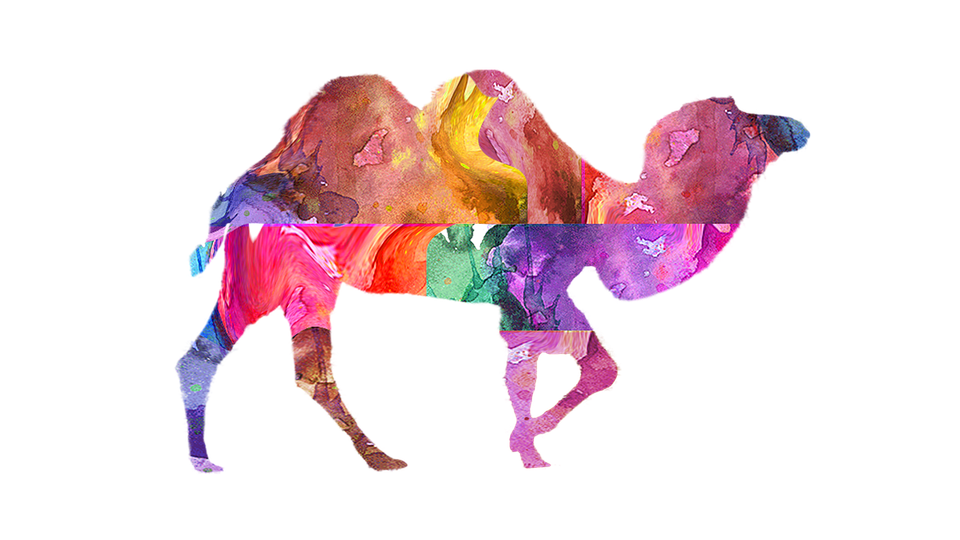
\includegraphics[width=0.78\linewidth]{Camel}\\
	First son gets $\frac{1}{2}$. Second son gets $\frac{1}{3}$. Third son gets $\frac{1}{9}$
\end{frame}
%----------------------------------------------------------------------------------------
\begin{frame}{Na{\"i}ve Method}
	\begin{itemize}
		\item Duplicate each player proportional to their ratio.\pause
		\item We will say that 
		\begin{itemize}
			\item Player 1 recieves $A_1$ allocation
			\item Player 2 recieves $A_2$ allocation
		\end{itemize}\pause
		\item Using the Even-Paz method, $\theta((\sum A)\log(\sum A))$ cuts are required.\newline
		\item We can do better!
	\end{itemize}
\end{frame}
%----------------------------------------------------------------------------------------
\begin{frame}{Cutting Ones}
	\begin{itemize}
		\item Similar to the cut-and-choose algorithm\pause
		\item Player 1 divides the cake into 1-sized parts
		\item Player 2 chooses $A_2$ of the 1-sized parts
	\end{itemize}
\end{frame}
%----------------------------------------------------------------------------------------
\begin{frame}{Ramsey Partitions}
	\begin{itemize}
		\item Ramsey theory is simply the study of edge colorings of complete graphs\pause
		\item We can observe this finding $R(3, 3)$\pause
	\end{itemize}
	The same property seen in Ramsey Theory can also be used to help partition
\end{frame}
%-------------------------------------------------------------------------------
\begin{frame}{Ramsey Partitions}
	\begin{itemize}
		\item Assume $A_1 < A_2$
		\item Player 1 cuts what they percieve to be $A_1$ of the cake.
		\item The smaller piece can be called $X_1$ and the larger piece can be called $X_2$
		\item If $\mu_2(X_2) < A_2$ (If the person thinks they got less than they were supposed to)
		\item Player 2 takes $X_1$ and division continues in the ratio $A_2 - A_1: A_1$ until no cake remains
	\end{itemize}
\end{frame}
%-------------------------------------------------------------------------------
%-------------------------------------------------------------------------------
\begin{frame}{Ramsey Partitions}
	\begin{itemize}
		\item This can be simplified using ramsey partitions
		\item Person 1 cuts the Ramsey Partitions of $\sum A$
		\item Person 2 marks all pieces $\mu_2(X_j) > \mu_1(X_j)$ (Everything they are willing to accept)\pause
		\begin{enumerate}
			\item If the sum of a subset of the marked pieces $= A_2$, we can give those pieces to Player 2 and give the rest to Player 1\pause 
			\item Otherwise, Player 1 may choose pieces summing to $A_1$ of the unmarked pieces. 
			\item This works because of the Ramsey Partitioning!
		\end{enumerate}
	\end{itemize}
\end{frame}
\end{document}
